\documentclass[../main.tex]{subfiles}

\begin{document}
\begin{questions}
	\question Two infinitely long grounded metal plates, at $y = 0$ and $y = a$, are connected at $x = \pm b$ by metal strips maintained at a constant potential $V_0$, (a thin layer of insulation at each corner prevents them from shorting out). Find the potential inside the resulting rectangular pipe. \label{q:q1}

	\begin{solution}
		We need to solve the equations
		\begin{align}
			\frac{\partial^2 V(x,y)}{\partial x^2} + \frac{\partial^2 V(x,y)}{\partial y^2} &= 0 && \text{Laplace's Equation}\\
			V(-b,y) &= V_0 && \text{Boundary Conditions}\label{eq:bc1}\\
			V(b,y) &= V_0\label{eq:bc2}\\
			V(x,0) &= 0\label{eq:bc3}\\
			V(x,a) &= 0\label{eq:bc4}
		\end{align}
		in the region $|x| \leq b$, $0\leq y\leq a$

		Using separation of variables, we know that the general solution can be written as
		\begin{align}
			V(x,y) = \sum_k (A_ke^{kx}+B_ke^{-kx})(C_k\cos{ky}+D_k\sin{ky})
		\end{align}
		Using \eqref{eq:bc3} and \eqref{eq:bc4}
		\begin{align}
			0 &= \sum_k C_k(A_ke^{kx}+B_ke^{-kx}) \label{eq:bc3cont}\\
			0 &= \sum_k (A_ke^{kx}+B_ke^{-kx})(C_k\cos{ka}+D_k\sin{ka}) \label{eq:bc4cont}
		\end{align}
		The trivial way to satisfy \eqref{eq:bc3cont} is $C_k = 0$ $\forall$ $k$\\
		Putting this back into \eqref{eq:bc4cont} we can see that $\sin ka = 0$ will satisfy it, hence only those $D_k$ terms are non zero, which satisfy $k=\frac{n\pi}{a}$\\
		We can thus index our coefficients by $n$ instead of $k$\\
		We get the general solution as
		\begin{align}
			V(x,y) = \sum_{n} (D_nA_ne^{n\pi\frac{x}{a}}+D_nB_ne^{-n\pi\frac{x}{a}})\sin(n\pi\frac{y}{a})
		\end{align}
		Using \eqref{eq:bc1} and \eqref{eq:bc2} we can see that $V(b,y) = V(-b,y)$
		\begin{align}
			\implies \sum_{n} A_ne^{n\pi\frac{b}{a}}+B_ne^{-n\pi\frac{b}{a}} &= \sum_n A_ne^{-n\pi\frac{b}{a}}+B_ne^{n\pi\frac{b}{a}}\\
			\implies \sum_n (A_n - B_n)(e^{n\pi\frac{b}{a}} + e^{-n\pi\frac{b}{a}}) &= 0\\
			\implies A_n &= B_n \text{ }\,\forall\,n
		\end{align}
		We can finally simplify our general solution as
		\begin{align}
			V(x,y) = \sum_{n=1}^{\infty} 2D_nA_n \cosh(n\pi\frac{x}{a})\sin(n\pi\frac{y}{a}) \label{eq:gen}
		\end{align}
		In order to solve this, we use \eqref{eq:bc2} (and write our coefficient as $K_n = 2D_nA_n$)
		\begin{align}
			V_0 &= \sum_{n=1}^{\infty} K_n \cosh(n\pi\frac{b}{a}) \sin(n\pi\frac{y}{a})
			\intertext{Using Fourier's trick}
			\int_{y=0}^{a} V_0 \sin(n'\pi\frac{y}{a})\,dy &= \sum_{n=1}^{\infty} K_n \cosh(n\pi\frac{b}{a}) \int_{y=0}^{a}\sin(n\pi\frac{y}{a})\sin(n'\pi\frac{y}{a})\,dy\\
			\implies \sum_{n=1}^{\infty} \frac{aK_n}{2} \cosh(n\pi\frac{b}{a})\delta_{nn'} &= 
			\begin{cases}
				0 & n' \text{ even}\\
				\frac{2aV_0}{n'\pi} & n' \text{ odd}
			\end{cases}\\
			\implies K_n &=
			\begin{cases}
				0 & n \text{ even}\\
				\frac{4V_0}{n\pi}\frac{1}{\cosh(n\pi\frac{b}{a})} & n \text{ odd}
			\end{cases}
		\end{align}
		Putting this back into \eqref{eq:gen},
		\begin{align}
			V(x,y) = \boxed{\frac{4V_0}{\pi}\sum_{n=1,3,5\dots} \frac{\cosh(n\pi\frac{x}{a})}{n\cosh(n\pi\frac{b}{a})}\sin(n\pi\frac{y}{a})}
		\end{align}
		We can indeed verify that this does satisfy the boundary conditions and the Laplace's equation, hence by Uniqueness theorem it must be the only solution
	\end{solution}

	\question A cubical box of side length $a$ consists of five metal plates welded together and grounded. The sixth plate at the top is insulated from the rest and maintained at $V_0$.
	\begin{parts}
		\part Argue that the potential at the centre should be $\frac{V_0}{6}$
		\begin{solution}
			Let us consider 6 seperate cases, where in the $i$\textsuperscript{th} case the $i$\textsuperscript{th} face is at potential $V_i$ and all others are at 0 potential (the charges on the faces arrange in such a way to facilitate this scenario in each case)\\
			It is not very difficult to see that each case is identical upto a rotation and scaling of the charges on each face. Thus the potential at the centre must be proportional to $V_i$ in the $i$\textsuperscript{th} case. Hence if we take a superposition of all cases, we can easily see that the resultant scenario in which $i$\textsuperscript{th} face is at $V_i$ must have the potential at centre $\propto \sum_i V_i$. If we take the case of all $V_i = V_0$, we can see that the proportionality constant is $\frac{1}{6}$\\
			Hence the potential at centre is $\frac{V_0}{6}$ when one face is held at $V_0$ and all others at $0$
		\end{solution}
		\newpage
		\part Find the potential inside the box.
		\begin{solution}
			We need to solve the equations
			\begin{align}
				\frac{\partial^2 V(x,y,z)}{\partial x^2} + \frac{\partial^2 V(x,y,z)}{\partial y^2}&+ \frac{\partial^2 V(x,y,z)}{\partial z^2} = 0 && \text{Laplace's Equation}\\
				V(x,y,a) &= V_0 && \text{Boundary Conditions}\label{eq:bc21}\\
				V(x,y,0) &= 0\label{eq:bc22}\\
				V(0,y,z)&= 0\label{eq:bc23}\\
				V(a,y,z)&= 0\label{eq:bc24}\\
				V(x,0,z)&= 0\label{eq:bc25}\\
				V(x,a,z)&= 0\label{eq:bc26}
			\end{align}
			For the region $0 \leq x,y,z \leq a$\\
			Using separation of variables we know that the general solution can be written as
			\begin{align}
				V(x,y,z) = \sum_{k,l} (A_k\cos kx + B_k\sin kx)(C_l \cos ly + D_l \sin ly)(E_{kl} e^{\sqrt{k^2+l^2}z} + K_{kl} e^{-\sqrt{k^2+l^2}z})
			\end{align}

			Applying \eqref{eq:bc23}, \eqref{eq:bc24}, \eqref{eq:bc25}, \eqref{eq:bc26}, we can see that
			\begin{align}
				A_k &= 0 \text{ } \forall \text{ } k\\
				B_k &= 0 \text{ } \forall \text{ } k\neq\frac{n\pi}{a}\\
				C_l &= 0 \text{ } \forall \text{ } l\\
				D_l &= 0 \text{ } \forall \text{ } l\neq\frac{m\pi}{a}
			\end{align}
			Applying \eqref{eq:bc22},
			\begin{align}
				E_{kl} + K_{kl} &= 0 \text{ } \forall \text{ } k,l
			\end{align}
			Thus we can write the general solution as (indexing the coefficients with $m,n$ instead of $k,l$)
			\begin{align}
				V(x,y,z) &= \sum_{n=1}^{\infty}\sum_{m=1}^{\infty} 2B_nD_mE_{nm}\sin(n\pi\frac{x}{a})\sin(m\pi\frac{y}{a})\sinh(\sqrt{n^2+m^2}\pi\frac{z}{a})
			\end{align}
			In order to solve this, we can use \eqref{eq:bc21} (and write the coefficient $K_nm=2B_nD_mE_{nm}$)
			\begin{align}
				V_0 &= \sum_{n=1}^{\infty}\sum_{m=1}^{\infty}K_{nm}\sin(n\pi\frac{x}{a})\sin(m\pi\frac{y}{a})\sinh(\sqrt{n^2+m^2}\pi)
			\end{align}
			Applying Fourier's trick,
			\begin{align}
				\int_{x=0}^{a}\int_{y=0}^{a}V_0 \sin(n'\pi\frac{x}{a})\sin(m'\pi\frac{y}{a}) &= \sum_{n=1}^{\infty}\sum_{m=1}^{\infty}K_{nm}\sinh(\sqrt{n^2+m^2}\pi)\\
				\times \int_{x=0}^{a}\int_{y=0}^{a}\sin(n\pi\frac{x}{a})&\sin(n'\pi\frac{x}{a})\sin(m\pi\frac{y}{a})\sin(m'\pi\frac{y}{a})\,dx\,dy
			\end{align}
			\begin{align}
				\implies \sum_{n=1}^{\infty}\sum_{m=1}^{\infty} \frac{a^2K_{nm}}{4}\sinh(\sqrt{n^2+m^2}\pi) \delta_{nn'}\delta_{mm'} &=
				\begin{cases}
					0 & n' \text{ even or } m' \text{ even}\\
					\frac{4a^2V_0}{\pi^2 n'm'} & n' \text{ odd and } m' \text{ odd} 
				\end{cases}
			\end{align}
			\begin{align}
				\implies K_{nm} &=
				\begin{cases}
					0 & n \text{ even or } m \text{ even}\\
					\frac{16V_0}{\pi^2 nm}\frac{1}{\sinh(\sqrt{n^2+m^2}\pi)} & n \text{ odd and } m \text{ odd} 
				\end{cases}
			\end{align}
			Thus we can write the solution as
			\begin{align}
				V(x,y,z) &= \frac{16V_0}{\pi^2}\sum_{n=1,3,5\dots}\sum_{m=1,3,5\dots} \frac{\sinh(\sqrt{n^2+m^2}\pi\frac{z}{a})}{nm\sinh(\sqrt{n^2+m^2}\pi)}\sin(n\pi\frac{x}{a})\sin(m\pi\frac{y}{a})
			\end{align}
			Summing it up numerically upto 49 terms gives us $0.166666666676V_0 \approx \frac{V_0}{6}$, confirming our ``guess''
		\end{solution}
	\end{parts}

	\question A rectangular pipe, running parallel to the z-axis (from $-\infty$ to $+\infty$), has three grounded metal sides, at $y = 0$, $y = a$, and $x = 0$. The fourth side, at $x = b$, is maintained at a specified potential $V_0(y)$. Develop a general formula for the potential inside the pipe.

	\begin{solution}
		We need to solve the equations
		\begin{align}
			\frac{\partial^2 V(x,y)}{\partial x^2} + \frac{\partial^2 V(x,y)}{\partial y^2} &= 0 && \text{Laplace's Equation}\\
			V(b,y) &= V_0(y) && \text{Boundary Conditions}\label{eq:bc31}\\
			V(0,y) &= 0\label{eq:bc32}\\
			V(x,0) &= 0\label{eq:bc33}\\
			V(x,a) &= 0\label{eq:bc34}
		\end{align}

		We can use separation of variables to write the general solution
		\begin{align}
			V(x,y) &= \sum_k (A_k e^{kx} + B_k e^{-kx})(C_k\cos ky + D_k\sin ky)
		\end{align}

		We can apply \eqref{eq:bc32}, \eqref{eq:bc33}, \eqref{eq:bc34} to get
		\begin{align}
			A_k + B_k &= 0 \,\forall\,k\\
			C_k &= 0 \,\forall\,k\\
			D_k &= 0 \,\forall\,k\neq\frac{n\pi}{a}
		\end{align}
		Thus we can write the general solution as
		\begin{align}
			V(x,y) &= \sum^{\infty}_{n=1} 2A_kD_k \sinh(n\pi\frac{x}{a})\sin(n\pi\frac{y}{a})
		\end{align}
		We use \eqref{eq:bc31} (Writing the coefficient as $K_n=2A_kD_k$)
		\begin{align}
			V_0(y) &= \sum_{n=1}^{\infty} K_n \sinh(n\pi\frac{b}{a})\sin(n\pi\frac{y}{a})\\
			\intertext{Applying Fourier's trick,}
			K_n &= \frac{2}{a}\frac{1}{\sinh(n\pi\frac{b}{a})}\int_{y=0}^{a} V_0(y)\sin(n\pi\frac{y}{a})\,dy
		\end{align}
		We can finally write the solution as
		\begin{align}
			V(x,y) &= \frac{2}{a}\sum_{n=1}^{\infty} \frac{\int_{y=0}^{a} V_0(y)\sin(n\pi\frac{y}{a})\,dy}{\sinh(n\pi\frac{b}{a})} \sinh(n\pi\frac{x}{a})\sin(n\pi\frac{y}{a})
		\end{align}
	\end{solution}

	\question Two infinitely long metal plates at $y = 0$ and $y = a$ are connected at $x = \pm b$ by metal strips maintained at a constant potential $V_0$. The potential on the bottom $(y = 0)$ is zero, however the potential on the top $(y =a)$ is a nonzero constant $V_1$. A thin layer of insulation at each corner prevents the plates from shorting out. Find the potential inside the resulting rectangular pipe.
	\begin{solution}
		To solve this we need to break this up into 2 situations
		\begin{center}
			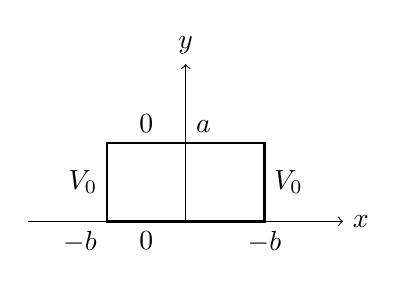
\begin{tikzpicture}
				\draw[->] (-2,0) -- (2,0) node[right]{$x$};
				\draw[->] (0,0) -- (0,2) node[above]{$y$};

				\draw[thick] (-1,0) node[below left]{$-b$} -- (-1,1) -- (0,1) node[above right]{$a$} -- (1,1) -- (1,0) node[below]{$-b$} -- cycle;

				\node at (1,0.5)[right] {$V_0$};
				\node at (-1,0.5)[left] {$V_0$};
				\node at (-0.5,1)[above] {$0$};
				\node at (-0.5,0)[below] {$0$};
			\end{tikzpicture}
			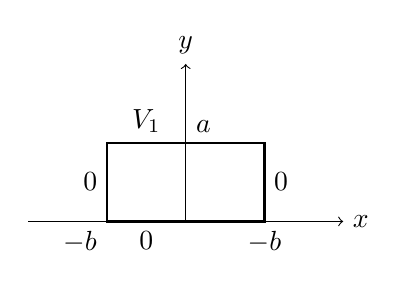
\begin{tikzpicture}
				\draw[->] (-2,0) -- (2,0) node[right]{$x$};
				\draw[->] (0,0) -- (0,2) node[above]{$y$};

				\draw[thick] (-1,0) node[below left]{$-b$} -- (-1,1) -- (0,1) node[above right]{$a$} -- (1,1) -- (1,0) node[below]{$-b$} -- cycle;

				\node at (1,0.5)[right] {$0$};
				\node at (-1,0.5)[left] {$0$};
				\node at (-0.5,1)[above] {$V_1$};
				\node at (-0.5,0)[below] {$0$};
			\end{tikzpicture}
		\end{center}
		\begin{center}
			Case I \hspace{3.25cm} Case II
		\end{center}
		We already know the solution to Case I (from Q\ref{q:q1}), 
		\begin{align}
			V_\text{I}(x,y) = \frac{4V_0}{\pi}\sum_{n=1,3,5\dots} \frac{\cosh(n\pi\frac{x}{a})}{n\cosh(n\pi\frac{b}{a})}\sin(n\pi\frac{y}{a})
		\end{align}

		Let us solve for Case II:\\
		We need to solve the equations
		\begin{align}
			\frac{\partial^2 V_\text{II}(x,y)}{\partial x^2} + \frac{\partial^2 V_\text{II}(x,y)}{\partial y^2} &= 0 && \text{Laplace's Equation}\\
			V_\text{II}(x,a) &= V_1 && \text{Boundary Conditions}\label{eq:bc41}\\
			V_\text{II}(x,0) &= 0\label{eq:bc42}\\
			V_\text{II}(y,-b) &= 0\label{eq:bc43}\\
			V_\text{II}(y,b) &= 0\label{eq:bc44}
		\end{align}
		in the region $|x| \leq b$, $0\leq y\leq a$\\
		Using separation of variables we can write the general solution as
		\begin{align}
			V_\text{II}(x,y) = \sum_k (A_k\cos kx + B_k \sin kx)(C_k e^{ky} + D_k e^{-ky})
		\end{align}
		Using \eqref{eq:bc42} we get
		\begin{align}
			C_k + D_k = 0
		\end{align}
		Thus our general solution simplifies to
		\begin{align}
			V_\text{II}(x,y) &= \sum_k 2C_k(A_k\cos kx + B_k \sin kx)\sinh(ky)
		\end{align}
		Putting \eqref{eq:bc43} and \eqref{eq:bc44} we get
		\begin{align}
			A_k\cos kb + B_k \sin kb &= 0\\
			A_k\cos kb - B_k \sin kb &= 0\\
			\implies A_k \cos kb = B_k \sin kb &= 0\\
			\implies A_k &= 0\, \forall\, k = \frac{2n\pi}{2b}\\
			B_k &= 0\,\forall\, k = \frac{(2n+1)\pi}{2b}\\
			A_k = B_k &= 0 \,\forall \, k \neq \frac{n\pi}{2b}
		\end{align}
		Hence we can write out our general solution as (indexing the coefficients accordingly)
		\begin{align}
			V_\text{II}(x,y) = 2C_1A_1 \cos(\pi\frac{x}{2b})\sinh(\pi\frac{y}{2b}) + 2C_2B_2 \sin(2n\pi\frac{x}{2b})\sinh(2\pi\frac{y}{2b}) \\
			+ 2C_3A_3 \cos(3n\pi\frac{x}{2b})\sinh(3\pi\frac{y}{2b})\dots
		\end{align}
		\begin{align}
			\implies V_\text{II}(x,y) = 2C_1A_1\sin(\pi\frac{x+b}{2b})\sinh(\pi\frac{y}{2b}) - 2C_2A_2\sin(2\pi\frac{x+b}{2b})\sinh(2\pi\frac{y}{2b})\\
			 + -2C_3A_3\sin(3\pi\frac{x+b}{2b})\sinh(3\pi\frac{y}{2b})\dots
		\end{align}
		Writing $\pm C_nA_n=K_n$,
		\begin{align}
			V_\text{II}(x,y) &= \sum^{\infty}_{n=1} K_n \sin(n\pi\frac{x+b}{2b})\sinh(n\pi\frac{y}{2b})
			\intertext{Using \eqref{eq:bc1}}
			V_1 &= \sum^{\infty}_{n=1} K_n \sin(n\pi\frac{x+b}{2b})\sinh(n\pi\frac{a}{2b})
			\intertext{Applying Fourier's trick,}
			K_n &=
			\begin{cases}
				0 & n \text{ even}\\
				\frac{4V_1}{n\pi}\frac{1}{\sinh(n\pi\frac{a}{2b})} & n \text{ odd}
			\end{cases}
		\end{align}
		Thus
		\begin{align}
			V_\text{II}(x,y) &= \frac{4V_1}{\pi}\sum_{n=1,3,5\dots} \frac{\sinh(n\pi\frac{y}{2b})}{n\sinh(n\pi\frac{a}{2b})}\sin(n\pi\frac{x+b}{2b})
			\intertext{We finally have}
			V(x,y) &= V_\text{I} + V_\text{II}\\
			&= \frac{4V_0}{\pi}\sum_{n=1,3,5\dots} \frac{\cosh(n\pi\frac{x}{a})}{n\cosh(n\pi\frac{b}{a})}\sin(n\pi\frac{y}{a})\\
			&+ \frac{4V_1}{\pi}\sum_{n=1,3,5\dots} \frac{\sinh(n\pi\frac{y}{2b})}{n\sinh(n\pi\frac{a}{2b})}\sin(n\pi\frac{x+b}{2b})
		\end{align}
	\end{solution}

	\question Consider a spherical surface of a large radius $R$, the potential on the spherical surface is given below. Using the separation of variables find the	potential $V(r,\theta)$ for $r \geq R$ upto order $\mathcal{O}(\frac{1}{r^6})$
	\begin{align*}
		V(R,\theta) &=
		\begin{cases}
			+V & 0 \leq \theta < \frac{\pi}{2}\\
			-V & \frac{\pi}{2} \leq \theta \leq \pi
		\end{cases}
	\end{align*}
	\begin{solution}
		We need to solve the equations (remembering that we have azimuthal symmetry)
		\begin{align}
			\frac{\partial}{\partial r}\left(r^2\frac{\partial V(r,\theta)}{\partial r}\right) &+ \frac{1}{\sin\theta}\frac{\partial}{\partial \theta}\left(\sin\theta\frac{\partial V(r,\theta)}{\partial \theta}\right) = 0 && \text{Laplace's Equation}\\
			V(R,\theta) &=
			\begin{cases}
				+V & 0 \leq \theta < \frac{\pi}{2}\\
				-V & \frac{\pi}{2} \leq \theta \leq \pi
			\end{cases} && \text{Boundary Conditions} \label{eq:rbc1}\\
			\lim_{r\to\infty}V(r,\theta) &= 0\label{eq:rbc2}
		\end{align}
		in the region $r\geq R$\\

		Using separation of variables we can write the general solution as
		\begin{align}
			V(r,\theta) &= \sum_{l=0}^{\infty} \left(A_l r^l + \frac{B_l}{r^{l+1}}\right)P_l(\cos\theta)
		\end{align}
		Using \eqref{eq:rbc2}, $A_l = 0$ $\forall$ $l$\\
		We can solve for the coefficients using \eqref{eq:rbc2}
		\begin{align}
			V(R,\theta) &= \sum_{l=0}^{\infty} \frac{B_l}{R^{l+1}}P_l(\cos\theta)\\
			\intertext{Applying Fourier's trick,}
			\int_{\theta=0}^{\pi} V(R,\theta)P_{l'}(\cos\theta)\sin\theta\,d\theta &= \sum_{l=0}^{\infty} \frac{B_l}{R^{l+1}} \int_{\theta=0}^{\pi} P_l(\cos\theta)P_{l'}(\cos\theta)\sin\theta\,d\theta
		\end{align}
		\begin{align}
			\implies V\int_{\theta=0}^{\frac{\pi}{2}} P_{l'}(\cos\theta)\sin\theta\,d\theta - V\int_{\theta=\frac{\pi}{2}}^{\pi} P_{l'}(\cos\theta)\sin\theta\,d\theta \\
			= \sum_{l=0}^{\infty} \frac{B_l}{R^{l+1}} \int_{\theta=0}^{\pi} P_l(\cos\theta)P_{l'}(\cos\theta)\sin\theta\,d\theta
		\end{align}
		\begin{align}
			\implies B_l &=
			\begin{cases}
				0 & l \text{ even}\\
				(2l+1)VR^{l+1} \int_{x=0}^{1}P_l(x)\,dx & l \text{ odd}
			\end{cases}
		\end{align}
		Thus our solution is
		\begin{align}
			V(r,\theta) &= V\sum_{l=1,3,5\dots} (2l+1)\frac{R^{l+1}}{r^{l+1}} P_l(\cos\theta)\int_{x=0}^{1}P_l(x)\,dx
		\end{align}
		We only need to calculate upto $l=5$ ($\mathcal{O}(\frac{1}{r^6})$)
		\begin{align}
			\int_{x=0}^{1} P_1(x)\,dx &= \frac{1}{2}\\
			\int_{x=0}^{1} P_3(x)\,dx &= -\frac{1}{8}\\
			\int_{x=0}^{1} P_5(x)\,dx &= \frac{1}{16}
		\end{align}
		Thus,
		\begin{align}
			V(r,\theta) &= V\left(\frac{3R^2}{2r^2}P_1(\cos\theta)-\frac{7R^4}{8r^4}P_3(\cos\theta)+\frac{11R^6}{16r^6}P_5(\cos\theta)\right) + \mathcal{O}(\frac{1}{r^8})
		\end{align}
	\end{solution}

	\newpage
	\question Let a sphere of radius $R$ have potential $V(R,\theta,\phi) = V_0 \cos^2 \theta$. Find
	the potential everywhere inside and outside the sphere.
	\begin{solution}
		Let us begin by calculating potential outside. As always, we have to solve
		\begin{align}
			\frac{\partial}{\partial r}\left(r^2\frac{\partial V_\text{out}(r,\theta)}{\partial r}\right) &+ \frac{1}{\sin\theta}\frac{\partial}{\partial \theta}\left(\sin\theta\frac{\partial V_\text{out}(r,\theta)}{\partial \theta}\right) = 0 && \text{Laplace's Equation}\\
			V_\text{out}(R,\theta) &= V_0 \cos^2 \theta && \text{Boundary Conditions}\label{eq:rbc61}\\
			\lim_{r\to\infty}V_\text{out}(r,\theta) &= 0\label{eq:rbc62}
		\end{align}
		in the region $r\geq R$
		We can write the general solution using separation of variables
		\begin{align}
			V_\text{out}(r,\theta) &= \sum_{l=0}^{\infty} \left(A_l r^l + \frac{B_l}{r^{l+1}}\right)P_l(\cos\theta)
		\end{align}
		Using \eqref{eq:rbc62}, $A_l = 0$\\
		We can solve for the coefficients using \eqref{eq:rbc61}
		\begin{align}
			V_0\cos^2\theta &= \sum_{l=0}^{\infty} \frac{B_l}{R^{l+1}} P_l(\cos\theta)
			\intertext{We can see that $B_l=0$ $\forall$ $l>2$ by observing the degree of $\cos\theta$ in the LHS}
			\implies V_0\cos^2\theta &= \frac{B_0}{R} + \frac{B_1}{R^2}\cos\theta + \frac{B_2}{2R^3}\left(3\cos^2\theta - 1\right)\\
			\intertext{Comparing the coefficients of like degrees of $\cos\theta$,}
			B_2 &= \frac{2V_0R^3}{3}\\
			B_1 &= 0\\
			B_0 &= \frac{V_0R}{3}\\
			\implies
			V_\text{out}(r,\theta) &= \frac{V_0R}{3r}\left(1+\frac{R^2}{r^2}\left(3\cos^2\theta-1\right)\right)
			\intertext{We can similarly find $V_\text{in}(r,\theta)$,}
			V_\text{in}(r,\theta) &= \frac{V_0}{3}\left(1+\frac{r^2}{R^2}\left(3\cos^2\theta-1\right)\right)
		\end{align}
	\end{solution}

	\question An uncharged, conducting sphere of radius $R$ is placed in a region where the electric field is uniform i.e. $\vec{E} = \vec{E}_0$. Can you guess whether $l$ value will be odd or even in potential outside the sphere? Find the electric field in
	the region after the sphere is put in place.
	\begin{solution}
		We can begin by observing that charges will distribute themeselves such that the charge density function will be odd in $\cos\theta$, and hence $l$ will also be odd\\
		WLOG, Let the external electric field be along $\hat{k}$, thus $\vec{E}_0 = E_0\hat{k}$. In spherical polar coordinates, $\vec{E}_0 = E_0 \cos\theta\,\hat{r} - E_0\sin\theta\,\hat{\theta}$\\
		This time we must be careful in setting the reference of potential, since we cannot set it to its usual at infinity (since everything near the sphere will have an infinite potential difference wrt infinity due to the constant $\vec{E}_0$ field). \\
		Remember that since our potential reference is now \textbf{not} at infinity, all of our intuitions regarding absolute potentials go out the window. Any potentials we must specify must also be accompanied by what they are in respect to. \\
		We can simply choose the reference to be the sphere surface itself. We can see that then the whole $xy$ plane will also be at 0 potential wrt the sphere ($\because$ due to symmetry, $\vec{E}\cdot\hat{r}=0$ on the $xy$ plane).\\
		Thus we observe that far away from sphere (where charges on sphere won't have any effect), $V = -E_0z = -E_0 r\cos\theta$
		Thus we need to solve the equations
		\begin{align}
			\frac{\partial}{\partial r}\left(r^2\frac{\partial V(r,\theta)}{\partial r}\right) &+ \frac{1}{\sin\theta}\frac{\partial}{\partial \theta}\left(\sin\theta\frac{\partial V(r,\theta)}{\partial \theta}\right) = 0 && \text{Laplace's Equation}\\
			V(R,\theta) &= 0 && \text{Boundary Conditions}\label{eq:rbc71}\\
			\lim_{r\to\infty}V(r,\theta) &= -E_0r\cos\theta\label{eq:rbc72}
		\end{align}
		in the region $r\geq R$
		As always, we can write the general solution using separation of variables
		\begin{align}
			V(r,\theta) = \sum_{l=0}^{\infty} \left(A_l r^l + \frac{B_l}{r^{l+1}}\right)P_l(\cos\theta)
		\end{align}
		Applying \eqref{eq:rbc71},
		\begin{align}
			B_l = -A_l R^{2l+1} \,\forall\,l
		\end{align}
		Applying \eqref{eq:rbc72}, we can see that $A_l = 0$ $\forall$ $l > 1$. Comparing coefficients,
		\begin{align}
			-E_0r\cos\theta &= A_0 + A_1r\cos\theta\\
			\implies A_0 &= 0\\
			A_1 &= -E_0
		\end{align}
		Putting it all together,
		\begin{align}
			V(r,\theta) &= -E_0\left(r-\frac{R^3}{r^2}\right)\cos\theta
		\end{align}
		Of course, remember that this potential is \textbf{in reference to the sphere}\\ 
		To find electric field,
		\begin{align}
			\vec{E} &= -\nabla V\\
			&= E_0\left(1+\frac{2R^3}{r^3}\right)\cos\theta\,\hat{r} - E_0\frac{1}{r}\left(r-\frac{R^3}{r^2}\right)\sin\theta\,\hat{\theta}\\
			&= \left(E_0\cos\theta\,\hat{r} - E_0\sin\theta\,\hat{\theta}\right) + E_0\frac{R^3}{r^3}\left(2\cos\theta\,\hat{r} + \sin\theta\,\hat{\theta} \right)
		\end{align}
		We can see that in addition to $\vec{E}_0$, a dipole field is induced by the sphere
	\end{solution}

	\question Suppose the potential $V_0(\theta)$ at the surface of the sphere is specified, and there is no charge outside or inside the sphere. Show that charge density on the surface of the sphere is given by
	\begin{equation*}
		\sigma(\theta) = \frac{\epsilon_0}{2R}\sum_{l=0}^{\infty} (2l+1)^2 C_l P_l(\cos\theta)
	\end{equation*}
	where $C_l$ is
	\begin{equation*}
		C_l = \int_{\theta=0}^{\pi} V_0(\theta)P_l(\cos\theta)\sin\theta\,d\theta
	\end{equation*}
	\begin{solution}
		We know that (after a simple application of separation of variables followed by Fourier's trick)
		\begin{align}
			V_\text{out}(r,\theta) &= \sum_{l=0}^{\infty} \frac{\int_{\theta=0}^{\pi}V_0(\theta)P_l(\cos\theta)\sin\theta\,d\theta}{r^{l+1}}\frac{(2l+1)R^{l+1}}{2}P_l(\cos\theta)\\
			&=  \sum_{l=0}^{\infty} \frac{C_l}{r^{l+1}}\frac{(2l+1)R^{l+1}}{2}P_l(\cos\theta)\\
			V_\text{in}(r,\theta) &= \sum_{l=0}^{\infty} \frac{\int_{\theta=0}^{\pi}V_0(\theta)P_l(\cos\theta)\sin\theta\,d\theta}{R^l}\frac{(2l+1)r^l}{2}P_l(\cos\theta)\\
			&= \sum_{l=0}^{\infty} \frac{C_l}{R^l}\frac{(2l+1)r^l}{2}P_l(\cos\theta)
		\end{align}
		We also know that
		\begin{align}
			\frac{\sigma(\theta)}{\epsilon_0} &= \left.-\frac{\partial V_\text{out}}{\partial r}\right|_{r=R} + \left.\frac{\partial V_\text{in}}{\partial r}\right|_{r=R}\\
			&= \sum_{l=0}^{\infty} \frac{(2l+1)C_lP_l(\cos\theta)}{2}\left(\frac{l}{R}+\frac{l+1}{R}\right)\\
			&= \frac{1}{2R}\sum_{l=0}^{\infty} (2l+1)^2 C_l P_l(\cos\theta)\\
			\implies \sigma(\theta) &= \frac{\epsilon_0}{2R}\sum_{l=0}^{\infty} (2l+1)^2 C_l P_l(\cos\theta)
		\end{align}
	\end{solution}
\end{questions}
\end{document}